\chapter{Generalization and Performance Evaluation}

\begin{multicols}{2}

\section{Overfitting and Underfitting}

\noindent Overfitting happens when test error rate begins to increase even though training error rate continues to decrease.

\noindent Underfitting happens when model is too simple, both training and test error rates are large. \\

\noindent In decision tree, the training error of a model can be reduced by increasing the model complexity. However, this action might leads to overfitting. The training error no longer provides a good estimate of how well the tree will perform on previously unseen records.

\section{Generalization Error}

\noindent Generalization error is a measure of how accurately an algorithm is able to predict outcome values of previously unseen data. To determine the right model complexity, we choose the model that produces the lowest generalization error. Since we do not have knowledge of test data, we can only estimate the generalization error of a model, using approaches such as Occam's Razor, pressimistic error estimate, and validation set. \\

\subsection{Occam's Razor}

Given two models of similar generalization errors, one should prefer the simpler model over the more complex model. For complex models, there is a greater chance that it was fitted accidentally by errors in data. Therefore, one should include model complexity when evaluating a model. 

\subsection{Pressimistic Error Estimate}

\noindent Explicityly computer generalization error as the sum of training error and a penalty term for model complexity. \\

\noindent Let $e(T)$ be the training errors, $e'(T)$ be the generalization errors, $\lambda$ be an tradeoff parameter, and $\Omega(T)$ be model complexity:

$$e'(T)=e(T) + \lambda \times \Omega(T)$$

\noindent In decision tree, we can define $\lambda=0.5$ and $\Omega(T)$ as the number of leaf nodes. 

\subsection{Validation Set}

Divide the original training data set into two smaller subsets. One is for training, and the other (validation set) is for estimating the generalization error. The complexity of the best model can be estimated by the performance of the model on validation set. 

\section{Prevent Overfitting}

\noindent In decision tree, we can prevent overfitting by pre-prunining (early stopping rule). Typical stopping conditions for a node:

\begin{itemize}
    \item Stop if all instances belong to the same class
    \item Stop if all the feature values are the same
    \item Stop if number of instances is less than some user-specified threshold
    \item Stop if class distribution of instances are independent of the available features
    \item Stop if expanding the current node does not improve impurity measures
\end{itemize}

\noindent We also can do post-pruning, by growing the decision tree to its entirely and trim the nodes of the decision tree in a bottom-up fashion. If generalization error improves after trimming, replace sub-tree by a new leaf node. Class label of leaf node is dtermined from majority class of instances in the sub-tree. 

\section{Model Evaluation}

\subsection{Metrics for Performance Evaluation}

\subsubsection{Confusion Matrix}
\begin{center}
\begin{tabular}{ | l | l | l | } 
    \hline
    Count & Predicted=YES & Predicted=NO \\
    \hline
    Actual=YES & TP & FN \\
    \hline
    Actual=NO & FP & TN \\
    \hline
\end{tabular}
\end{center}

\subsubsection{Accuracy}

$$Accuracy=\frac{TP + TN}{TP + FN + FP + TN}$$

\noindent In many real-world applications, data sets may have imbalanced class distributions. Accuracy measure treats every class as equally important, it may not be suitable for analyzing imbalanced data sets, where the rare class is considered more interesting than the majority class. \\

\subsubsection{Precision, Recall, F1-measure}

\noindent Precision is to measure among all the predicted positive instances, how many are true positive:

$$Precision,p=\frac{TP}{TP + FP}$$

\noindent Recall is to measure among all true positive instances, how many are predicted correctly by the classifier:

$$Recall,r=\frac{TP}{TP+FN}$$

\noindent A good model should have both high precision and recall. Recall and precision can be summarized into another metric known as $F_1measure$:

$$F_1measure=\frac{2PR}{P+R}$$

\subsubsection{Receiver Operating Characteristic}

\noindent ROC (Receiver Operating Characteristic) is a graphical approach to displaying the trade-off between true positive rate and false positive rate of a classifier.

\noindent True Positive Rate (TPR):
$$TPR = \frac{TP}{TP+FN}$$

\noindent False Positive Rate (FPR):
$$FPR = \frac{FP}{TN + FP}$$

\begin{center}
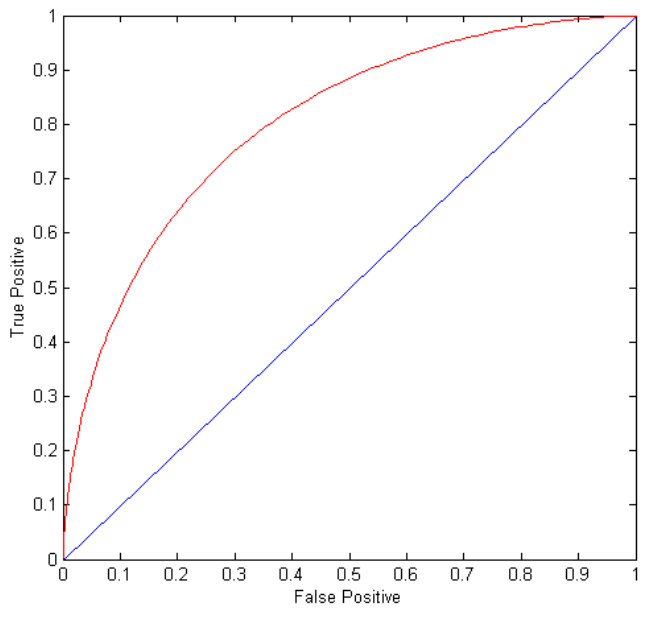
\includegraphics[width=5cm, height=5cm]{roc_curve}
\end{center}

\noindent The ROC curve:

\begin{itemize}
    \item (0,0) declare everything to be negative class
    \item (1,1) declare everything to be positive class
    \item (1,0) ideal
    \item On the diagonal line, random guessing
    \item Below diagonal line, prediction is opposite of the true class
\end{itemize}

\subsection{Methods for Performance Evaluation}

\begin{description}
    \item[Holdout] reserve 2/3 for training and 1/3 for testing, sampled without replacement
    \item[Random subsampling] repeated holdout. The average accuracy for all samples are calculated. 
    \item[Cross validation] partition data into $k$ disjoint subsets of the same size. Hold aside one group for testing and use the rest to build model. The performance is evaluate based on the accuracy of $k$ models on test set. 
    \item[Leave-One-Out] k-fold cross-validation, with $k=n$
    \item[Bootstrap] similar to holdout, but sampling with replacement
\end{description}

\end{multicols}